\chapter{The Network Stack} % Main chapter title

\label{Chapter4} % For referencing the chapter elsewhere, use \ref{Chapter1} 

\lhead{Chapter 4. The Network Stack} % This is for the header on each page - perhaps a shortened title

In this chapter, we take a look at how we implemented the UDP stack for Atmosphere. Since Atmosphere is not ready yet, we build a standalone network stack that runs in the userspace and evaluate its performance. We use a custom userspace network driver (based on Ixy) to process raw ethernet frames sent to and from the network stack. This driver is shared across applications just as it would be in the real Atmosphere.

\begin{figure}[!htbp]
	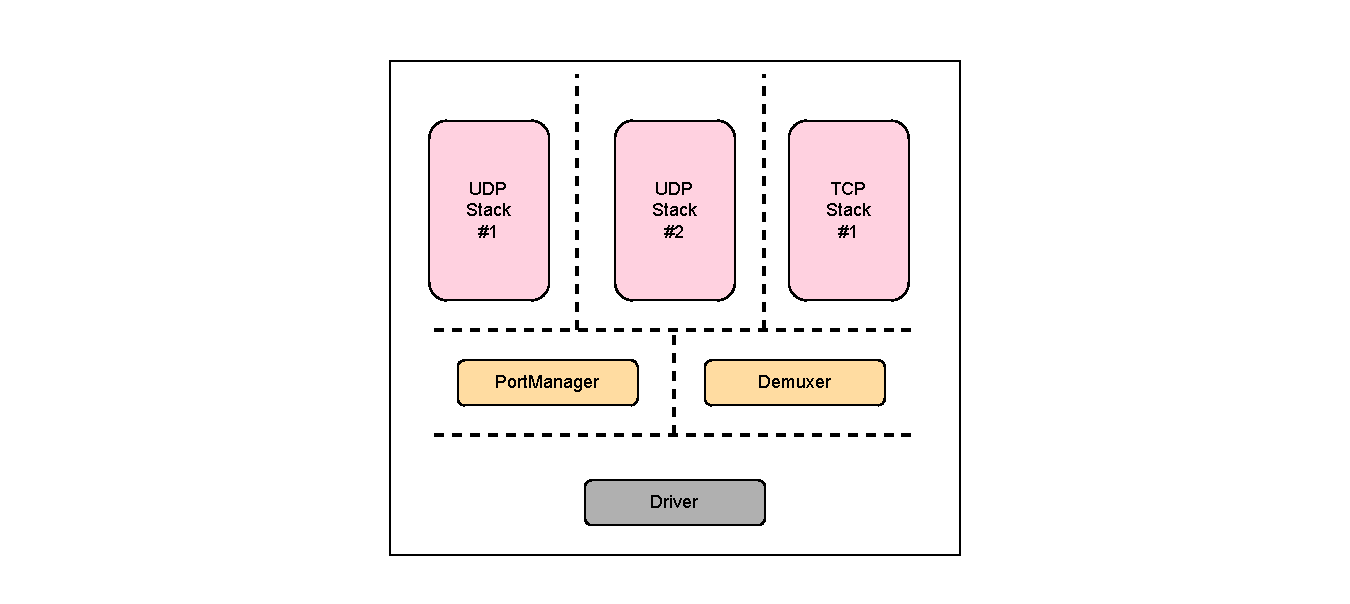
\includegraphics[width=1.0\columnwidth]{figures/network-design.pdf}
\caption{Atmosphere network stack design}
	\label{fig:network-design}
\end{figure}

\section{Driver for the Network Card}

Ixy is a network driver implemented in the userspace for Intel's Ixgbe family of network cards that shows how network cards work at the driver level. It is implemented in a fashion similar to DPDK and Snabb. We use a version of Ixy written in Rust and modify it to fit the design of our network stack. Two main limitations of Ixy (as per our design) are: (1) it handles allocations in the driver and (2) received packets cannot be reused as transmit packets. (2) is important as for a lot of applications (e.g. MICA), we want to be able to flip headers in a received packet and send it back to the client. 

The major modifications we make to ixy.rs are:
\begin{itemize}
    \item{Change the way packets are allocated. We get rid of the huge-pages backed Mempool and allow packets to be discretely allocated. DMA mapping is done for every packet. }
\item{Receive queues do not allocate packets themselves. Instead, the application supplies a batch of allocated buffers which is used to read packets from the NIC. This relieves the NIC from having to do any allocations. }
\end{itemize}

On testing with an Ixgbe NIC with a line rate of 10GB/s, we see no drop in performance after our modifications.

\subsection{Packet Storage}
As mentioned above, packets are stored in a DMA-mapped page-sized buffer. Listing \ref{listing:1} illustrates the Packet struct and how it is allocated. While allocating a page for each packet is wasteful in terms of memory, there is no discernible change in performance in processing packets. This also enables the NIC to interleave packets from different applications in the same queue without crossing any isolation boundaries.

\begin{listing}[!htbp]
\begin{minted}[fontsize=\footnotesize, frame=lines, framesep=2mm]{Rust}
#[repr(C, align(PAGESZ))]
pub(crate) struct PacketBuffer {
    data: [u8; PAGESZ]
}

pub struct Packet {
    pub(crate) addr_virt: *mut u8,
    pub(crate) addr_phys: usize,
    pub(crate) len: usize,
    pub(crate) data: Box<PacketBuffer>,
}

pub fn alloc_pkt(len: usize) -> Option<Packet> {
    let mut buffer = Box::new(PacketBuffer{ data: [0;PAGESZ] });
    let addr_virt = buffer.data.as_mut_ptr();
    let mut p = Packet {
        data: buffer,
        addr_virt,
        len,
        addr_phys: 0,
    };
    match vfio_map_dma(p.addr_virt as usize, PAGESZ) {
        Ok(addr_phys) => {
            p.addr_phys = addr_phys;
            Some(p)
        }
        Err(e) => {
            error!("{}", e);

            None
        }
    }
}
\end{minted}
\caption{Packet storage in modified ixy}
\label{listing:1}
\end{listing}


\section{Port Manager}
The PortManager handles all allocations and deallocations of ports and keeps track of which stacks they are bound to. To be able to formally verify its implementation in the future, the interface it exposes is minimal and it only interacts with the opaque identifiers rather than actual types. 
UDP stacks can be identified by using only the destination port in an incoming packet (we assume that the device is connected to a single IPv4 interface for simplicity). But for TCP connections, since a single port can handle multiple connections, and every connection is handled by a different stack, we maintain a separate flow table for matching TCP connections.
The PortManager also helps the demuxer identify which stack a packet should go to, or if it is to be dropped.

\section{Demuxer}
The demuxer matches incoming packets with a destination stack and and returns free buffers from the NIC to the stack that owns them. The demuxer can also maintains private queues for applications that are not actively receiving packets but have incoming packets destined to them. 
On receiving a packet, the demuxer parses the protocol and the destination port (or the TCP 5-tuple) and use the PortManger to find the destination stack. If the packet is matched, we push it to the private queue. The next time the application calls receive, the private queue is emptied and the packets are returned to the stack. If the private queue for a stack is saturated, incoming packets are simply dropped.

\subsection{Packet Flipping}
Since the buffers for a receive call come from a stack, and since all packets received might not be destined to the same stack, the demuxer can flip a buffer from its private queue so that the application does not lose a free buffer to the demuxer. This is done by popping a buffer from a private queue and flipping it with the received buffer. The application can then get a free buffer in return for the buffer it contributed for the packet of another stack.

\subsection{UDP Interface}
We provide a low level interface for the application to interface applications with the udp protocol. We provide a \lstinline{UdpStack} interface that exposes two main methods: \lstinline{tx_batch()} and \lstinline{rx_batch()} both of which are non-blocking and interact with discrete packet buffers. Note that this is currently a low level interface requiring the user to setup a static arp table and routes in the ipv4 table themeselves. this can be changed in the future when the stack is integrated with atmosphere. We also provide a convenience function called \lstinline{prepare_batch()} that lets users provide a buffer and fills discrete packets with all required headers and the data from the given buffer. For ease of manipulating packet headers, we provide a \lstinline{UDPPacketRepr} representation which has setters and getters for protocol headers. \ref{listing:2} illustrates the code for a simple UDP echo server.

\begin{listing}[!htb]
\begin{minted}[fontsize=\footnotesize, frame=lines, framesep=2mm]{Rust}
pub fn main() {
    let mut stack = create_udp_stack(Ipv4Address::new(10, 0, 0, 2), 5000);
    let mut free_bufs: VecDeque<RawPacket> = VecDeque::with_capacity(NUM_PACKETS);
    let mut recv_batch: VecDeque<UdpPacketRepr> = VecDeque::with_capacity(NUM_PACKETS);
    let mut send_batch: VecDeque<UdpPacketRepr> = VecDeque::with_capacity(NUM_PACKETS);

    let mut num_recvd;

    loop {
        (num_recvd, recv_batch, free_bufs) = stack
            .recv_batch(recv_batch, free_bufs, BATCH_SIZE)
            .expect("failed to receive packets");
        recv_batch.drain(..num_recvd).for_each(|mut pkt| {
            // flip source and destination
            pkt.set_udp_packet(|mut udp| {
                let src = udp.get_source();
                let dst = udp.get_destination();
                udp.set_destination(src);
                udp.set_source(dst);
            });
            pkt.set_ip_packet(|mut ip| {
                let src = ip.get_source();
                let dst = ip.get_destination();
                ip.set_destination(src);
                ip.set_source(dst);
            });
            send_batch.push_back(pkt);
        });
        (send_batch, free_bufs) = stack
            .send_batch(send_batch, free_bufs)
            .expect("failed to sent packets");
    }
}
\end{minted}
\caption{Example UDP echo server}
\label{listing:2}
\end{listing}
